\chapter{Background on cryptography} \label{cryptography background}

The Finnish Data Protection Act and the GDPR regulate the controller and processor of any personal data to implement proper technical and organization measures in terms of security, while taking into account the level of risk related to the nature of the data stored.
Health related data is considered a special category of personal data by the GDPR and therefore should be handled with extra caution.
The GDPR mentions pseudonymization and encryption of personal as options for improving the security of sensitive data.
As health data is considered very sensitive, appropriate cautions should be taken when storing and processing it, including the two tools mentioned by the GDPR.
\cite{gdpr}

This chapter explains the basics of cryptography, unfortunately this requires a small bit of mathematics.
Different cryptographic systems are also introduced here, as well as options for implementing cryptography in a public cloud.

\section{Cryptography}

Cryptography is the science of keeping messages secure.
Encryption is a part of cryptography which in layman's terms means sending text in the form of secret writing.
The message to be sent is first converted into an indiscernible form via cryptographic methods.
The original message is called the plaintext and the encrypted message is called the ciphertext.
The message is then delivered over computer networks.
The receiver then reverses the ciphertext using the reverse of the same cryptographic method, resulting in the exact same message that was sent by the sender.
Using cryptography only the sender and the receiver can read the original message and no third party can intercept it or tamper with it on the way.
\cite{applied-crypto}

The main job for cryptography is to achieve the following traits: confidentiality, integrity and availability.
These concepts are often referred to as the CIA triad.
The meaning for each of them is the following: \cite{crypto-principles}
\begin{itemize}
    \item Confidentiality: Only the original sender and the recipient can read the message.
    No third party can eavesdrop on the communications.
    \item Integrity: The message is transmitted through the communication channel as-is without any third party tampering with it.
    \item Availability: The information is readily available without unnecessary delays to all authorized parties.
\end{itemize}

The three previously discussed concepts of cryptography are visualized in Fig \ref{fig:cryptography-concepts}.

\begin{figure}[!htb]
\centering
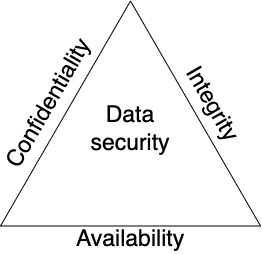
\includegraphics[scale=1.0]{cia-triad}
\caption{Visualization of the CIA triad, the three concepts of data security}
\label{fig:cryptography-concepts}
\end{figure}

The CIA triad is quite a well established list of traits.
However, some in the cryptography space feel that additional concepts are necessary.
The additional concepts often listed are the following \cite{crypto-principles}:
\begin{itemize}
    \item Authenticity: The message can be confirmed authentic using cryptographic measures.
    The users communicating are also validated as who they claim to be.
    \item Accountability: The actions of an individual are traceable to them.
    Because no system is truly secure, it is beneficial to be able to trace the source of a possible security breach.
\end{itemize}

A cryptographic algorithm, also called a cipher, is a mathematical function used for encrypting and decrypting a message.
There are often two separate functions: one for encrypting and the other for decrypting.
\cite{applied-crypto}

A cryptographic algorithm which encryption is based on keeping how the function works a secret is called a restricted algorithm.
Restricted algorithms have been used historically, but they are quite inadequate by today's standards.
If the secret is revealed at any point, every user must change to an entirely new algorithm.
\cite{applied-crypto}
% security by obscurity

Modern cryptographic solutions solve this problem using keys.
This key can be any value on a large range of values, called the keyspace.
Both operations, encryption and decryption, use this key as part of the function.
Some algorithms use a different encryption and decryption keys.
The security of these algorithms is based entirely on the secrecy of the key or keys.
The details of the algorithm can therefore be made public and analyzed.
Leaking of the algorithm is no longer an issue, as long as the eavesdropper does not gain access to the keys.
\cite{applied-crypto}

Cryptographic algorithms can be divided into two general categories: symmetric and asymmetric, also known as public-key.
An algorithm being symmetric means that the encryption key can be calculated from the decryption key and vice versa.
In most cases, the encryption and decryption key is the same.
Before beginning secure communication on a single-key algorithm, the sender and receiver must agree on a key.
The key is central to the security of the communication, keeping it a secret makes the communications a secret.
\cite{applied-crypto}

Public-key algorithms are characterized by using a separate key for both encryption and decryption.
The decryption key cannot be calculated from the encryption key (in a reasonable time).
The encryption key is often called the public key.
The decryption key is referred to as the private key.
The algorithms are named "public-key" because the encryption key can be made public.
Anyone can use the public key to encrypt a message, but only a specific person with the private key can decrypt it.
It is also possible an algorithm uses the private key to encrypt and the public key to decrypt data.
An example of such use case would be digital signatures, which prove a specific person's signature to be genuine and the authenticity and integrity of the message.
\cite{applied-crypto}

The most relevant public-key algorithms use prime numbers as the basis of their functionality.
The primes used are very, very large: many hundred digits long.
\cite{practical-crypto}
Factoring a number means finding its prime factors.
The core idea in using primes in cryptography, is that factoring a number is very time-consuming.
For example, in 1993 a 120-digit hard number was factored in 3 months of real time using 825 mips-years\footnote{
Mips-year is an unit used to measure computational effort in cryptography.
One mips-year is the amount of work performed by a single computer in a year, operating at one million operations per second or 1 MIPS.
}
of computing power.
On the other hand, generating prime numbers and multiplying them is easy.
Answering the question "is \textit{n} prime?" is a lot easier than answering the question "what are the factors of \textit{n}?" because the former is just a yes/no question.
\cite{applied-crypto}
Multiplication is more work than addition, for example, but it is still relatively easy for a computer to perform.
\cite{practical-crypto}

\section{Pseudonymization}

Pseudonymization means changing all identifiable personal data such as e-mail addresses, names and IP addresses for aliases.
The information can no longer be connected to a specific individual without additional data.
Pseudonymization is highly recommended by the GDPR.
Although the process of pseudonymization is reversible, it significantly lowers the risk of leaking sensitive data.
\cite{gdpr}
The irreversible process of changing identifiable personal data for an alias is called anonymisation.

The GDPR suggests organizations to implement pseudonymization, however it does not define a technique or process for it.
The GDPR only gives us the end goal of pseudonymization: making the data unable to be attributed to a natural person.
By this definition, encryption fulfills this goal.
\cite{pseudonymisation}

% Voi miettiä, meneekö vähän syvemmällekin vaikkapa esimerkin kautta
%

\section{Envelope encryption}

Envelope encryption is an encryption strategy used with large scale applications.
It allows for both, centralized safekeeping of encryption keys as well as encrypting a large amount of data.
Envelope encryption uses multiple layers of keys by encrypting a key with another key.
The key that is used to encrypt another key is called the \textit{key encryption key} (KEK).
The key that encrypts the data itself is called the \textit{data encryption key} (DEK).
The process of decrypting a DEK with a KEK is also called wrapping, and is visualized in \ref{fig:envelope-encryption-key}.
Decrypting the data with the DEK is visualized in \ref{fig:envelope-encryption-data}.
\cite{googlecloud}

Google lists best practices for working with DEKs and KEKs.
DEKs should be generated locally by the program handling the data and always encrypted at rest.
For easy access, the DEK can be stored near the data it encrypts.
KEKs should be managed and stored centrally, for example on Google Cloud Platform's Cloud Key Management Service (KMS).
The granularity of KEKs should be considered by workload, the same KEK can be used for data the workload is responsible for.
KEKs should be rotated regularly and also after any suspicious activity.
A new DEK should be used every time new data is stored.
This also means DEKs will never have to be rotated.
The same DEK should never be used for two different users.
\cite{googlecloud}

The security advantage of envelope encryption is in the key encryption key and using a different data encryption key for each chunk of data.
Even if a malicious actor were to gain access to a plaintext DEK, they would only be able to decrypt a small chunk of data.
The malicious actor would need both: the centrally stored KEK as well as the database with the DEKs to decrypt all the data.
\cite{googlecloud}

\begin{figure}[!htb]
\centering
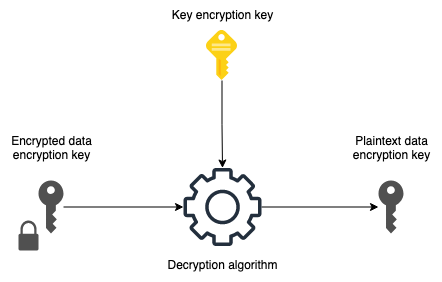
\includegraphics[scale=0.8]{envelope-encryption-key}
\caption{Visualization of decrypting a data encryption key with a key encryption key}
\label{fig:envelope-encryption-key}
\end{figure}

\begin{figure}[!htb]
\centering
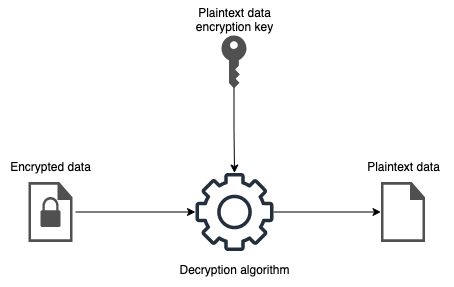
\includegraphics[scale=0.8]{envelope-encryption-data}
\caption{Visualization of decrypting data with a plaintext data encryption key}
\label{fig:envelope-encryption-data}
\end{figure}